\section{Choice of drone}\label{s:vores_drone}
For the purpose of this project a multirotor drone will be chosen. The drone chosen for the project was a self built drone.
A Quanum Outlaw 270 Racing Drone Frame Kit with 305 mm in diameter was chosen as the main body for the drone system, the full drone is shown on figure \ref{fig:TheChosenOne}. The reason for choosing a larger drone body and the reason for more powerful motors will be used is because of the possibility of lifting a heavier payload, such as a micro controller and sensors. 

\begin{figure}[H]
    \centering
    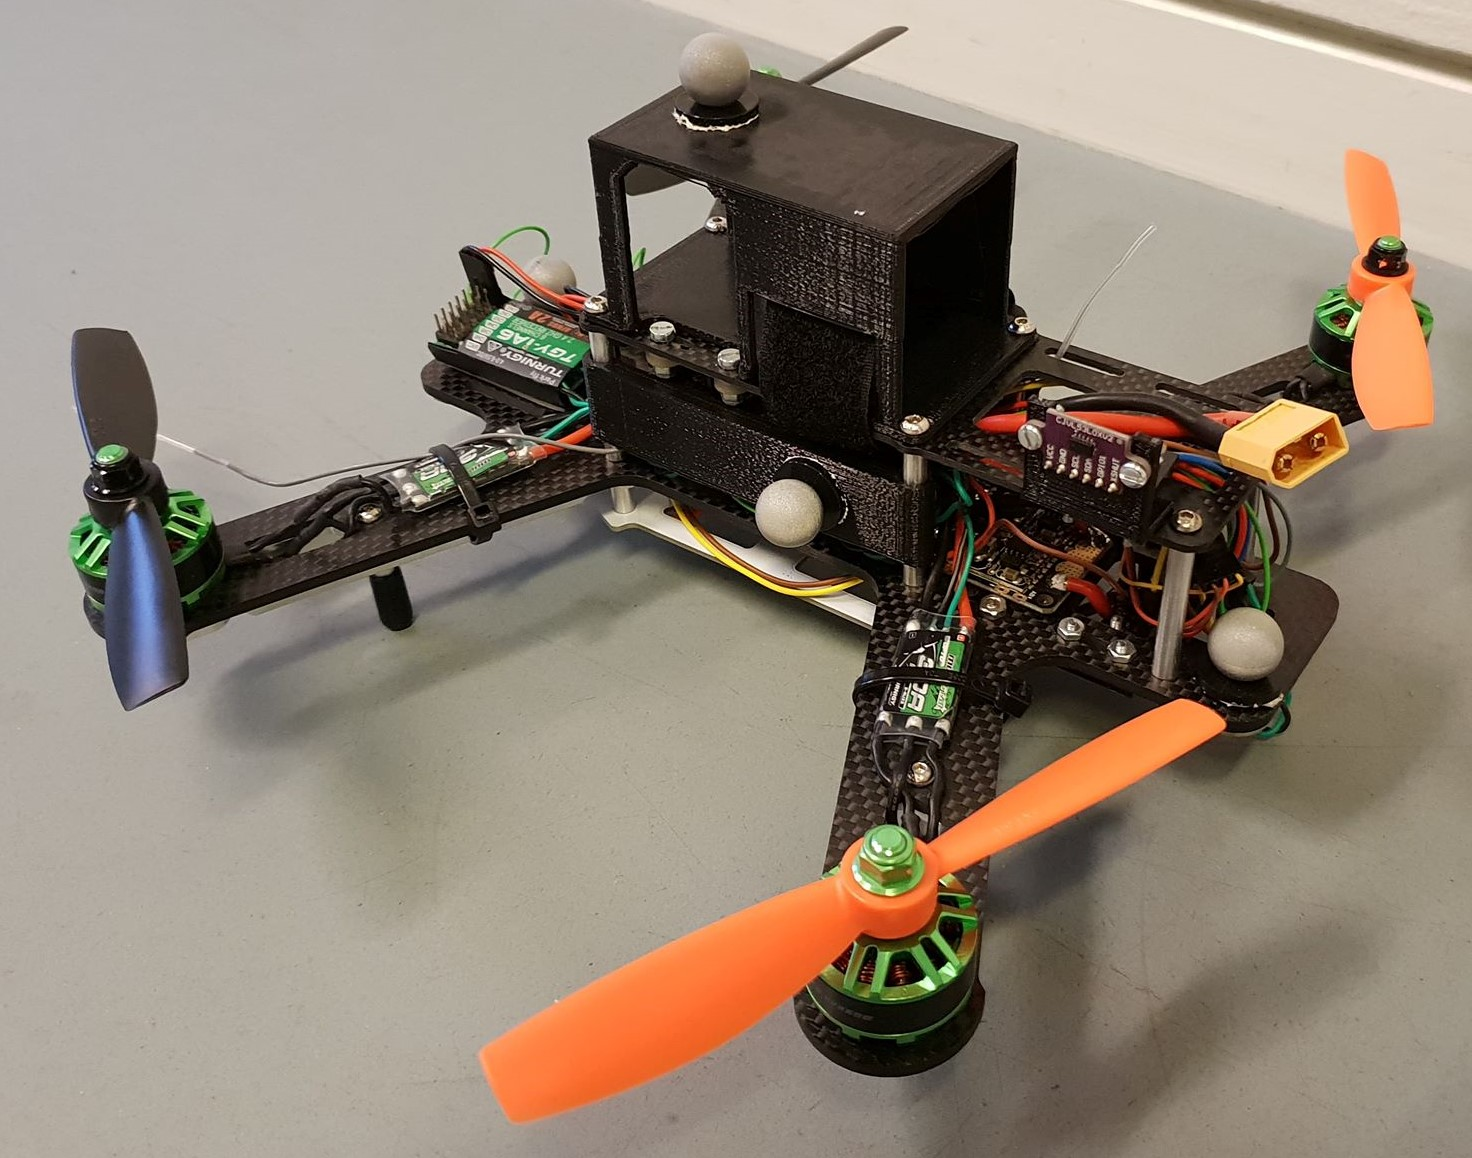
\includegraphics[width=0.5\textwidth]{figures/ch_intro/TheChosenOne2.jpg}
    \caption{A picture of the chosen drone for this project.}
    \label{fig:TheChosenOne}
\end{figure}

\subsection*{Composition of quadcopter parts}
The composition of the different parts on the quadcopter is illustrated on figure \ref{fig:blockdiagramDrone} and the list of components can be seen in the table \ref{tab:drone_element}. 

\begin{figure}[H]
    \centering
    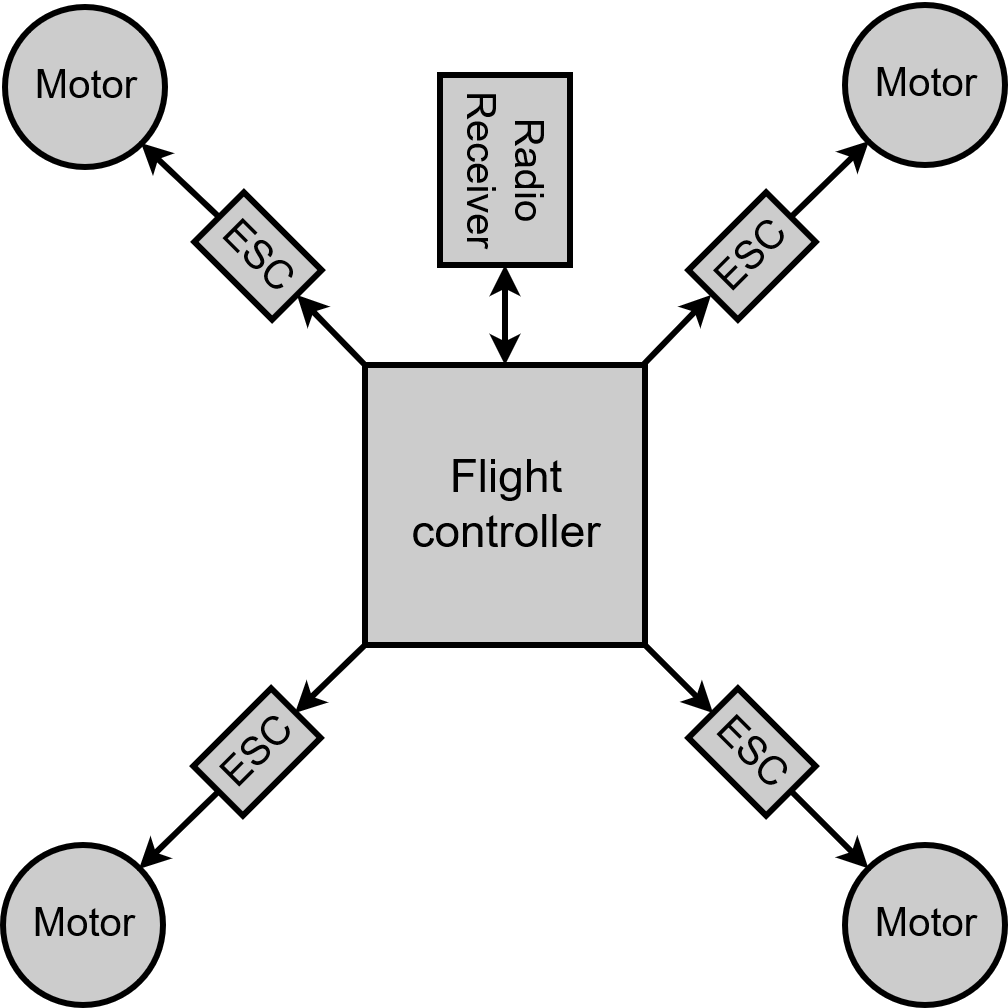
\includegraphics[width=0.5\textwidth]{figures/ch_intro/BlockdiagramOfTheDrone.png}
    \caption{Block diagram of the quadcopters individual parts connection.}
    \label{fig:blockdiagramDrone}
\end{figure}

\begin{table}[H]
\caption{List of the components used for the drone.}\label{tab:drone_element}
\begin{tabular}{|c|p{12cm}|}
\hline
\textbf{Quantity} & \textbf{Item} \\ \hline
1 x  & \textbf{Frame kit:} Quanum Outlaw 270 Racing Drone Frame Kit \\ \hline
1 x & \textbf{Flight controller:} Skyline32 Acro Flight Controller w/Baseflight  Cleanflight \\ \hline
4 x & \textbf{Motor:} MultiStar Viking 2206-2600kv Brushless Outrunner Drone Racing Motor (CCW) \\ \hline
1 x & \textbf{Battery} Turnigy Heavy Duty 2200mAh 4S 60C Lipo Pack w/XT60U Connector \\ \hline
1 x & \textbf{Controller unit} Turnigy TGY-i6 AFHDS Transmitter and 6CH Receiver (Mode 2) \\ \hline
4 x & \textbf{ESC:} Turnigy MultiStar 32bit 30A Race Spec ESC 2~4S NAKED (OPTO) \\ \hline
4 x & \textbf{Propellers:} Diatone Bull Nose Plastic Propellers \\ \hline
\end{tabular} 
\end{table}